\documentclass[10pt,a4paper,final]{article} %draft

\usepackage[english, russian]{babel}

\usepackage{geometry}
%\usepackage[a4paper,left=2cm,right=2cm,top=2cm,bottom=2cm,bindingo ffset=0cm]{geometry}

\usepackage[T2A]{fontenc}
\usepackage[utf8]{inputenc}

\usepackage[utf8]{inputenc}

\usepackage[final]{pdfpages}

\usepackage{textcomp,enumitem}

\usepackage{amsmath,amsthm,amssymb}

\usepackage{longtable}
\usepackage{array}
\usepackage{adjustbox}

\usepackage{wrapfig}



\usepackage{listings}
\usepackage{xcolor}
\usepackage{caption}

\definecolor{codegray}{rgb}{0.95,0.95,0.95}
\definecolor{codepurple}{rgb}{0.58,0,0.82}
\definecolor{codegreen}{rgb}{0,0.5,0} % зеленый цвет
\definecolor{codeblue}{rgb}{0,0,0.5} % синий цвет
\definecolor{codestring}{rgb}{0.64,0.08,0.08} % цвет строк


\lstset{
	language=haskell,
	extendedchars=true,
	literate=
	{а}{{\selectfont\char224}}1
	{б}{{\selectfont\char225}}1
	{в}{{\selectfont\char226}}1
	{г}{{\selectfont\char227}}1
	{д}{{\selectfont\char228}}1
	{е}{{\selectfont\char229}}1
	{ж}{{\selectfont\char230}}1
	{з}{{\selectfont\char231}}1
	{и}{{\selectfont\char232}}1
	{й}{{\selectfont\char233}}1
	{к}{{\selectfont\char234}}1
	{л}{{\selectfont\char235}}1
	{м}{{\selectfont\char236}}1
	{н}{{\selectfont\char237}}1
	{о}{{\selectfont\char238}}1
	{п}{{\selectfont\char239}}1
	{р}{{\selectfont\char240}}1
	{с}{{\selectfont\char241}}1
	{т}{{\selectfont\char242}}1
	{у}{{\selectfont\char243}}1
	{ф}{{\selectfont\char244}}1
	{х}{{\selectfont\char245}}1
	{ц}{{\selectfont\char246}}1
	{ч}{{\selectfont\char247}}1
	{ш}{{\selectfont\char248}}1
	{щ}{{\selectfont\char249}}1
	{ъ}{{\selectfont\char250}}1
	{ы}{{\selectfont\char251}}1
	{ь}{{\selectfont\char252}}1
	{э}{{\selectfont\char253}}1
	{ю}{{\selectfont\char254}}1
	{я}{{\selectfont\char255}}1
	{А}{{\selectfont\char192}}1
	{Б}{{\selectfont\char193}}1
	{В}{{\selectfont\char194}}1
	{Г}{{\selectfont\char195}}1
	{Д}{{\selectfont\char196}}1
	{Е}{{\selectfont\char197}}1
	{Ж}{{\selectfont\char198}}1
	{З}{{\selectfont\char199}}1
	{И}{{\selectfont\char200}}1
	{Й}{{\selectfont\char201}}1
	{К}{{\selectfont\char202}}1
	{Л}{{\selectfont\char203}}1
	{М}{{\selectfont\char204}}1
	{Н}{{\selectfont\char205}}1
	{О}{{\selectfont\char206}}1
	{П}{{\selectfont\char207}}1
	{Р}{{\selectfont\char208}}1
	{С}{{\selectfont\char209}}1
	{Т}{{\selectfont\char210}}1
	{У}{{\selectfont\char211}}1
	{Ф}{{\selectfont\char212}}1
	{Х}{{\selectfont\char213}}1
	{Ц}{{\selectfont\char214}}1
	{Ч}{{\selectfont\char215}}1
	{Ш}{{\selectfont\char216}}1
	{Щ}{{\selectfont\char217}}1
	{Ъ}{{\selectfont\char218}}1
	{Ы}{{\selectfont\char219}}1
	{Ь}{{\selectfont\char220}}1
	{Э}{{\selectfont\char221}}1
	{Ю}{{\selectfont\char222}}1
	{Я}{{\selectfont\char223}}1,
	%	{|}{{\textbar}}1,
	%	{||}{{\textbar\textbar}}1
	%	{\&}{{\string&}}1
	%	{==}{{\string==}}1
	%	{\string\\}{{\string\\}}1,
	numbers=left,
	stepnumber=1,
	firstnumber=1,
	numberstyle=\tiny,
	basicstyle=\ttfamily\footnotesize,
	breakatwhitespace=false,
	breaklines=true,
	postbreak=\mbox{\textcolor{gray}{$\hookrightarrow$}}, % Символ переноса строки
	captionpos=b,
	keepspaces=true,
	showspaces=false,
	showstringspaces=false,
	showtabs=false,
	tabsize=2,
	frame=single,
	keywordstyle=\color{codeblue}, % ключевые слова
	commentstyle=\color{codegreen}, % комментарии
	stringstyle=\color{codestring}, % строки
	%identifierstyle=\color{green}, % стиль для переменных
	backgroundcolor=\color{codegray},
}
%\usepackage{fancyvrb}

%\usepackage{fancyhdr}

%\usepackage{upgreek}

%\usepackage{tipa}

%\usepackage{tikz}

%\usepackage{graphicx}

%\usepackage{pgfplots}

\usepackage{indentfirst}

%\usepackage{gensymb}

%\usepackage{amssymb}

%\usepackage{pdfpages}

\usepackage[unicode, pdftex, colorlinks, urlcolor=blue]{hyperref}

%\usepackage[T2A]{fontenc}


\usepackage{tabularx}
\usepackage{multirow}

\usepackage{booktabs} % для стильных линий таблицы



\usepackage{graphics}

\linespread{1.5}

\pagestyle{plain}

%\usepackage{listings} 
%\usepackage{moreverb} 

%\setlist[enumerate,itemize]{leftmargin=1.2cm} %отступ в перечислениях

\hypersetup{
	colorlinks=true,
	linkcolor=black,
	%allcolors=[RGB]{0 0 0}}
	}
	%\lstloadlanguages{ [LaTeX] TeX}
	
	\lstloadlanguages{ [LaTeX] TeX}
	
	
	
	\textheight=24cm 
	\textwidth=16cm
	\oddsidemargin=0pt 
	\topmargin=-1.5cm
	\parindent=24pt 
	\parskip=0pt 
	\tolerance=2000 
	\flushbottom 
	
	%\usepackage[font=scriptsize]{caption}
	\usepackage[labelsep=period]{caption}
	
	\begin{document}
\thispagestyle{empty}

\begin{center}
	{\Large МИНОБРНАУКИ РОССИИ}\\
	~\\
	{\large ФЕДЕРАЛЬНОЕ ГОСУДАРСТВЕННОЕ БЮДЖЕТНОЕ ОБРАЗОВАТЕЛЬНОЕ УЧРЕЖДЕНИЕ ВЫСШЕГО ПРОФЕССИОНАЛЬНОГО ОБРАЗОВАНИЯ}\\
	~\\
	{\Large \bf <<САНКТ-ПЕТЕРБУРГСКИЙ ПОЛИТЕХНИЧЕСКИЙ УНИВЕРСИТЕТ ПЕТРА ВЕЛИКОГО>>}\\
	~\\
	{\large Институт компьютерных наук и кибербезопасности}\\
	{\large Высшая школа технологий искусственного интеллекта}\\
	{\large Направление 02.03.01 Математика и компьютерные науки}\\
	~\\
	~\\
	~\\
	~\\
	{\Large \bf Отчет по практическому заданию №3}\\
	{\Large по дисциплине <<Функциональное программирование>> }\\
	~\\
	~\\
	
	%{\Large }\\
	%	{\Large \bf }\\ 	
	
	~\\
	~\\
	~\\
	~\\
	~\\
	~\\
	~\\
	~\\
	~\\
	{\large Обучающийся: \underline{\hspace{3.5cm}} \qquad\qquad Гладков И.А.}\\
	~\\
	{\large Руководитель: \underline{\hspace{3.5cm}} \hspace{15mm} Моторин Д.Е.}\\
	~\\
	~\\
\end{center}
\begin{flushright}
	
	«\underline{\hspace{1cm}}»\underline{\hspace{3cm}}20\underline{\hspace{0.7cm}}г.
\end{flushright}
~\\
\begin{center}
	{\large Санкт-Петербург, 2024}
\end{center}
\newpage

\tableofcontents

\newpage

\section* {Введение}
\addcontentsline{toc}{section}{Введение}
\par В данном отчете описан результат выполнения практического задания №3. Целью которого было шифрование текста биографии предоставленного ученного в изображение и дешифрирование текста из  изображения.

Шифрование текста происходит в два этапа: сначала текст шифруется шифром с использованием кодового слова (кодовое слово выбирает пользователь), затем зашифрованный текст записывается в один, два, ... , восемь последних битов каждого байта изображения, на усмотрение пользователя. Дешифрирование выполняется с помощью ключа и количество бит, записанных в названии изображения, в котором зашифрован текст.

Практическая работа выполняется на языке Haskell 9.4.8 в текстовом редакторе Visual Studio Code 1.95.3

\newpage
\section {Постановка задач}

Для выполнения практического задания необходимо выполнить следующие задачи:
\begin{enumerate}
	\item Создать проект в \texttt{stack}
	\item Все чистые функции записать в библиотеку \texttt{Lib.hs} и ограничить доступ к вспомогательным функциям
	\item Использовать do-нотацию для работы с внешними файлами.
	\item Использовать портрет Алонзо Черча в формате \texttt{.bmp} и текст с его биографией, содержащим в себе не менее 1000 символов без пробелов. 
	\item Реализовать функцию кодирующую текст в изображение с помощью шифра с использование кодового слова, где кодовое слово задает пользователь. Далее ключ шифру записывается в имя файла.
	\item Написать функцию расшифровывающую текст из изображения используя ключ из имени файла и сохраняющую результат в отдельный текстовый файл.
	\item Создать функции шифрующие текст в последний бит каждого байта, последние два бита каждого байта, ..., все биты в байте изображения. 
\end{enumerate}

\newpage
\section{Математическое описание}
\subsection{Шифр с использованием кодового слова}

Шифр с использованием кодового слова представляет собой модифицированную версию шифра подстановки, в котором каждый символ открытого текста шифруется с использованием соответствующего символа кодового слова. Кодовое слово повторяется, если его длина меньше длины текста. Такой подход обеспечивает псевдослучайность шифрования и делает метод более устойчивым к криптоанализу по сравнению с простыми шифрами сдвига.

Пусть $P$ — открытый текст, $C$ — шифротекст, а $K$ — кодовое слово. Если каждому символу алфавита сопоставить его порядковый номер, начиная с 0, то шифрование и дешифрование можно описать следующими формулами модульной арифметики:

\[
c_i = (p_i + k_{(i \mod m)}) \mod n
\]
\[
p_i = (c_i - k_{(i \mod m)}) \mod n
\]

где: \\
$p_i$ — $i$-й символ открытого текста, \\
$c_i$ — $i$-й символ шифротекста, \\
$k_j$ — $j$-й символ кодового слова, \\
$n$ — мощность алфавита, \\
$m$ — длина кодового слова.

Для расшифрования используется обратное преобразование, основанное на вычитании значения символа кодового слова.




\newpage
\section{Особенности реализации}
\subsection{Исходное изображение и текст}

В работе использовались 24-разрядное изображение формата \texttt{.bmp}  и текстовый файл содержаший 1085 символов без пробелов. 

Портер и биография Алонзо Черча представлены ниже:\\



\begin{wrapfigure}{r}{0.4\textwidth} % {r} - картинка справа, 0.4\textwidth - ширина картинки
	\centering
	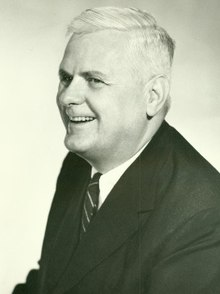
\includegraphics[width=0.3\textwidth]{img/Alonzo_Church} % пример изображения
	
\end{wrapfigure}

Alonzo Church's parents were Mildred Hannah Letterman Parker and Samuel Robbins Church. His father was a judge. He was a student at Princeton receiving his first degree, an A.B., in 1924, then his doctorate three years later. His doctoral work was supervised by Veblen, and he was awarded his doctorate in 1927 for his dissertation entitled Alternatives to Zermelo's Assumption. While he was still working for his doctorate he married Mary Julia Kuczinski at Princeton in 1926. They had three children, Alonzo Jr, Mary Ann and Mildred. Church spent two years as a National Research Fellow, one year at Harvard University then a year at Gottingen and Amsterdam. He returned to the United States becoming Assistant Professor of Mathematics at Princeton in 1929.He was promoted to Associate Professor in 1939 and to Professor in 1947, a post he held until 1961 when he became Professor of Mathematics and Philosophy. In 1967 he retired from Princeton and went to the University of California at Los Angeles as Kent Professor of Philosophy and Professor of Mathematics. He continued teaching and undertaking research at Los Angeles until 1990 when he retired again, twenty-three years after he first retired! In 1992 he moved from Los Angeles to Hudson, Ohio, where he lived out his final three years.\\



\subsection{Основной модуль}

Основной модуль программы, \texttt{Main}, реализует меню для выбора действий: шифрования и расшифровки текста, а также управления путями к файлам и изображениями. В нем определены функции для работы с изображениями и текстами, а также для шифрования и расшифровки данных.

\begin{lstlisting}[language=Haskell, caption=Основной модуль программы]
	module Main (main) where
	
	import Lib
	import Codec.Picture
	import System.IO
	import Control.DeepSeq (deepseq)
	import Control.Exception (IOException, try)
	
	main :: IO ()
	main = do
	menu
	
	menu :: IO()
	menu = do
	putStrLn "Choose the action:"
	putStrLn "[1] - encrypting text"
	putStrLn "[2] - decrypting text"
	putStrLn "[0] - Bye!"
	input <- getLine
	if null input  -- Проверка на пустой ввод
	then do
	putStrLn "You must choose a valid option. Please try again."
	menu
	else do
	let n = read input :: Int
	case n of    
	1 -> do
	menuEncrypting
	putStrLn "---------------------------------"
	menu
	2 -> do
	menuDecrypting
	putStrLn "---------------------------------"
	menu
	0 -> putStrLn "Exiting..."
	_ -> do
	putStrLn "Invalid choice. Try again."
	putStrLn "---------------------------------"
	menu
\end{lstlisting}

\subsubsection{Шифрование текста}

Функция \texttt{menuEncrypting} обрабатывает процесс шифрования текста. Пользователь может указать путь к изображению, текстовому файлу и ключ шифрования. После получения всех данных, программа шифрует текст и сохраняет изображение с зашифрованными данными.

\begin{lstlisting}[language=Haskell, caption=Шифрование текста]
	menuEncrypting :: IO()
	menuEncrypting = do
	putStrLn "write path to the image (default \"files\\Alonzo_Church.bmp\")"
	input <- getLine
	let path = if null input then  "files\\Alonzo_Church.bmp" else input :: String
	key = getKey path
	eimg <- readImage path
	case eimg of
	Left err -> putStrLn $ "Failed to open image: " ++ err
	Right dynImg -> do 
	let img = convertRGB8 dynImg   
	binaryImage = imageToBinary img
	height = imageHeight img
	width = imageWidth img
	putStrLn $ "image size: " ++ (show width) ++ " x " ++ (show height)
	
	putStrLn "write path to .txt file (default \"files\\Alonzo Church's Biography.txt\")"
	inputF <- getLine
	let fileName = if null inputF then  "files\\Alonzo Church's Biography.txt" else inputF :: String
	openning <- try (readFile fileName) :: IO (Either IOException String)
	case openning of
	Left ex -> putStrLn $ "Failed to open file: " ++ show ex
	Right text -> do
	let binaryEncodedText = binaryEncoding $ encoding key text
	putStrLn $ "Lenght of text in bits: " ++ show  (length binaryEncodedText)
	putStrLn "Write Key for encoding (default \"Haskell\"):"
	input1 <- getLine
	let key = if null input1 then "Haskell" else input1 :: String
	
	putStrLn "Write count of bits (default 4):"
	input2 <- getLine
	let inp = if null input2 then 4 else read input2 :: Int
	count <- check inp 
	
	putStrLn "Coordinates for encrypting write coordinate x (default 0):"
	inputX <- getLine
	let coordX = if null inputX then 0 else read inputX :: Int
	putStrLn "Coordinates for encrypting write coordinate y (default 0):"
	inputY <- getLine
	let coordY = if null inputY then 0 else read inputY :: Int
	
	(x, y) <- coordinate (coordX, coordY, width, height, count, (length binaryEncodedText))
	
	let encryptedText = encrypting binaryImage binaryEncodedText count x y
	img' = binaryStringToImage encryptedText width height
	img'' = ImageRGB8 img'
	putStrLn "text is encrypting..."
	encryptedText `deepseq` putStrLn "text encrypted..."
	putStrLn "image is saving..."
	let filePath = "files/" ++ key ++ "_" ++ show count ++ ".bmp"
	saveBmpImage filePath img''
	putStrLn $ "Image saved to \"" ++ filePath ++ "\""
\end{lstlisting}

\subsubsection{Дешифровка текста}

Функция \texttt{menuDecrypting} обрабатывает процесс дешифровки текста. Пользователь может указать путь к зашифрованному изображению и файл для сохранения расшифрованного текста. Программа извлекает данные из изображения, расшифровывает их и сохраняет в файл.

\begin{lstlisting}[language=Haskell, caption=Дешифровка текста]
	menuDecrypting :: IO()
	menuDecrypting = do
	putStrLn "write path to the image (default \"files\\Haskell_4.bmp\")"
	input <- getLine
	let path = if null input then  "files\\Haskell_4.bmp" else input :: String
	key = getKey path
	eimg <- readImage path
	case eimg of
	Left err -> putStrLn $ "Failed to open image: " ++ err
	Right dynImg -> do 
	let img = convertRGB8 dynImg   
	binaryImage = imageToBinary img
	(key, bits) = getKeyBits path
	bText = decrypting binaryImage bits
	binaryDecodedText = binaryDecoding bText
	decodedText = decoding key binaryDecodedText
	putStrLn $ "write path to save decrypted image (default \"files\\decrypdedImage.txt\")"
	input1 <- getLine
	let fileName = if null input1 then "files\\decrypdedImage.txt" else input1 :: String
	
	putStrLn "image is decrypting..."
	bText `deepseq` putStrLn "image decrypted..."
	putStrLn "text is saving..."
	file <- openFile fileName WriteMode
	hPutStr file decodedText
	hClose file
	putStrLn $ "Decrypted image saved to \"" ++ fileName ++ "\""
\end{lstlisting}







\subsection{Библиотека \texttt{Lib.hs}}

В данном разделе приведены основные функции, реализованные в проекте на языке Haskell.

\subsubsection{Функция \texttt{removeDublicates}}

Удаляет дубликаты из строки. Функция использует вспомогательную рекурсивную функцию для обхода всех символов в строке.

\begin{lstlisting}[language=Haskell, caption=Функция удаления дубликатов]
	removeDublicates :: String -> String  
	removeDublicates = removeDublicates' []
	where
	removeDublicates' :: String -> String -> String
	removeDublicates' _ [] = []
	removeDublicates' seen (x:xs)
	| x `elem` seen = removeDublicates' seen xs
	| otherwise = x : removeDublicates' (x:seen) xs
\end{lstlisting}

\subsubsection{Функция \texttt{convertText}}

Преобразует текст с одного алфавита в другой, используя таблицу преобразования (список пар символов).

\begin{lstlisting}[language=Haskell, caption=Функция конвертации текста]
	convertText :: String -> String -> String -> String
	convertText [] _ _ = []
	convertText (c:cs) alphabet newAlphabet =
	let converted = case lookup c (zip alphabet newAlphabet) of
	Just x -> x
	Nothing -> c
	in converted : convertText cs alphabet newAlphabet
\end{lstlisting}

\subsubsection{Функция \texttt{createAlphabet}}

Создает алфавит на основе переданного ключа, добавляя в него уникальные символы.

\begin{lstlisting}[language=Haskell, caption=Функция создания алфавита]
	createAlphabet :: String -> String 
	createAlphabet [] = " !\"#$%&'()*+,-./0123456789:;<=>?@ABCDEFGHIJKLMNOPQRSTUVWXYZ[\\]^_`abcdefghijklmnopqrstuvwxyz{|}"
	createAlphabet str = 
	let newStr = str ++ " !\"#$%&'()*+,-./0123456789:;<=>?@ABCDEFGHIJKLMNOPQRSTUVWXYZ[\\]^_`abcdefghijklmnopqrstuvwxyz{|}"
	in  removeDublicates newStr
\end{lstlisting}

\subsubsection{Функция \texttt{encoding}}

Шифрует текст с помощью кодировки, основанной на кодовом слове.

\begin{lstlisting}[language=Haskell, caption=Функция шифрования]
	encoding :: String -> String -> String
	encoding key text =
	let alphabet = createAlphabet [] 
	newAlphabet = createAlphabet key
	in convertText text alphabet newAlphabet
\end{lstlisting}

\subsubsection{Функция \texttt{decoding}}

Декодирует текст с использованием кодового слова, возвращая исходный текст.

\begin{lstlisting}[language=Haskell, caption=Функция декодирования]
	decoding :: String -> String -> String
	decoding key text = 
	let alphabet = createAlphabet key
	defaultAlphabet = createAlphabet []
	in convertText text alphabet defaultAlphabet 
\end{lstlisting}

\subsubsection{Функции для работы с двоичным кодом}

Эти функции позволяют преобразовывать числа, символы и строки в двоичную форму и обратно.

\begin{lstlisting}[language=Haskell, caption=Функции для работы с двоичным кодом]
	toBinary :: Int -> Vector Char 
	toBinary n = V.fromList (replicate (8 - length bin) '0') V.++ V.fromList bin
	where bin = showIntAtBase 2 intToDigit n ""
	
	fromBinary :: Vector Char -> Int 
	fromBinary str 
	| V.null str = 0 
	|otherwise = num + fromBinary str'
	where 
	num = if V.head str == '1' then 2 ^ (length str - 1) else 0 
	str' = V.tail str
	
	charToBinary :: Char -> Vector Char
	charToBinary c = toBinary $ ord c
	
	charFromBinary :: Vector Char -> Char
	charFromBinary c =  chr $ fromBinary c 
	
	binaryEncoding :: String -> Vector Char
	binaryEncoding [] = V.empty
	binaryEncoding (c:cs) = charToBinary c V.++ binaryEncoding cs
	
	binaryDecoding :: Vector Char -> String
	binaryDecoding str
	| V.null str = []
	| V.length str < 8 = []
	| otherwise = charFromBinary (V.take 8 str) : binaryDecoding (V.drop 8 str)
\end{lstlisting}

\subsubsection{Функции для работы с изображениями}

Эти функции преобразуют пиксели и изображения в двоичный формат и обратно.

\begin{lstlisting}[language=Haskell, caption=Функции для работы с изображениями]
	pixelToBinary :: PixelRGB8 -> Vector Char
	pixelToBinary (PixelRGB8 r g b) = toBinary (fromIntegral r) V.++ toBinary (fromIntegral g) V.++ toBinary (fromIntegral b) 
	
	imageToBinary :: Image PixelRGB8 -> Vector Char
	imageToBinary img = V.concat [pixelToBinary (pixelAt img x y) | y <- [0..height-1], x <- [0..width-1]]
	where 
	width = imageWidth img
	height = imageHeight img
\end{lstlisting}

\subsubsection{Функции для работы с двоичной строкой и изображениями}

Эти функции обрабатывают двоичные строки, преобразуя их в изображения и обратно.

\begin{lstlisting}[language=Haskell, caption=Функции для работы с двоичными строками и изображениями]
	binaryStringToColor :: Vector Char -> Word8
	binaryStringToColor str = fromIntegral $ foldl (\acc x -> acc * 2 + digitToInt x) 0 str
	
	binaryStringToImage :: Vector Char -> Int -> Int -> Image PixelRGB8
	binaryStringToImage str width height = 
	let size = height * width * 3 * 8
	newStr = takeCurrentSize str size
	pixelRenderer x y =
	let index = (y * width + x) * 3 * 8
	r = binaryStringToColor (V.take 8 (V.drop index newStr))
	g = binaryStringToColor (V.take 8 (V.drop (index + 8) newStr))
	b = binaryStringToColor (V.take 8 (V.drop (index + 16) newStr))
	in PixelRGB8 r g b
	in generateImage pixelRenderer width height
\end{lstlisting}

\subsubsection{Функция \texttt{getKey}}

Извлекает ключ из пути к файлу.

\begin{lstlisting}[language=Haskell, caption=Функция получения ключа]
	getKey :: String -> String
	getKey path = 
	takeWhile (/= '.') (reverse (takeWhile (\c -> c /= '\\' && c /= '/') (reverse path)))
\end{lstlisting}

\subsubsection{Функция \texttt{getKeyBits}}

Извлекает ключ и количество бит из пути к файлу.

\begin{lstlisting}[language=Haskell, caption=Функция получения ключа и битов]
	getKeyBits :: String -> (String, Int)
	getKeyBits path = 
	let fileName = takeWhile (/= '.') (reverse (takeWhile (\c -> c /= '\\' && c /= '/') (reverse path)))
	key = takeWhile (/= '_') fileName
	bits = takeWhile (/= '.') (filter  (/= '_') (dropWhile (/= '_') fileName))
	bits' = read bits::Int
	in (key, bits')
\end{lstlisting}

\subsubsection{Функция \texttt{encrypting}}

Шифрует изображение, используя двоичный код и заданное количество бит.

\begin{lstlisting}[language=Haskell, caption=Функция шифрования изображения]
	encrypting :: Vector Char -> Vector Char -> Int -> Int -> Int -> Vector Char
	encrypting img str count x y = runST $ do
	let indx = 0
	len = length img
	str' = takeCurrentSize str (len `div` 8 * count)
	result <- MV.new (len)
	
	let go indx
	| indx < x * y + y = do
	V.forM_ (V.fromList [0..7]) $ \i -> do
	let val = if str' !! indx == '1' then 1 else 0
	MV.write result indx val
	go (indx +1)
	go indx
	return result
\end{lstlisting}


\newpage
\section{Результаты}

Запускаем программу, для зашифровки текста выбираем \texttt{<<encrypting text>>} и пишем путь к изображению, путь к текстовому файлу, кодовое слово и количество бит.
Для расшифровки текста выбираем \texttt{<<decrypting text>>}, пишем путь к зашифрованному тексту, то есть изображению, после пишем куда сохранить текст после расшифровки.

Ниже приведены результаты программы шифрования текста в изображение с количеством битов от 1 до 8 и кодовым словом \texttt{<<Haskell>>}. При расшифровки каждого изображения получался изначальный текст.

\begin{figure}[h!]
	\centering
	\begin{minipage}{0.3\textwidth}
		\centering
		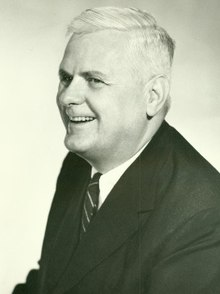
\includegraphics[width=\linewidth]{img/Alonzo_Church}
		\caption{Оригинальное изображение}
	\end{minipage}
	\hspace{0.02\textwidth}
	\begin{minipage}{0.3\textwidth}
		\centering
		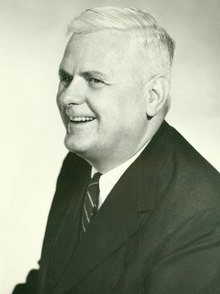
\includegraphics[width=\linewidth]{img/Haskell_1}
		\caption{Шифрование текста в 1 бит байта}
	\end{minipage}
	\hspace{0.02\textwidth}
	\begin{minipage}{0.3\textwidth}
		\centering
		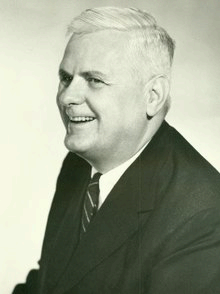
\includegraphics[width=\linewidth]{img/Haskell_2}
		\caption{Шифрование текста в 2 бита байта}
	\end{minipage}
\end{figure}


\begin{figure}[h!]
	\centering
	\begin{minipage}{0.3\textwidth}
		\centering
		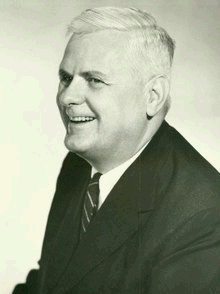
\includegraphics[width=\linewidth]{img/Haskell_3}
		\caption{Шифрование текста в 3 бита байта}
	\end{minipage}
	\hspace{0.02\textwidth}
	\begin{minipage}{0.3\textwidth}
		\centering
		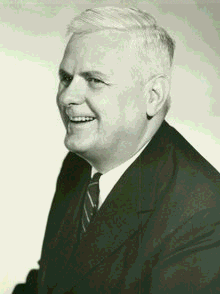
\includegraphics[width=\linewidth]{img/Haskell_4}
		\caption{Шифрование текста в 4 бита байта}
	\end{minipage}
	\hspace{0.02\textwidth}
	\begin{minipage}{0.3\textwidth}
		\centering
		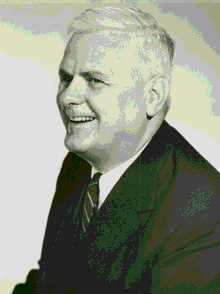
\includegraphics[width=\linewidth]{img/Haskell_5}
		\caption{Шифрование текста в 5 битов байта}
	\end{minipage}
\end{figure}

\newpage

\begin{figure}[h!]
	\centering
	\begin{minipage}{0.3\textwidth}
		\centering
		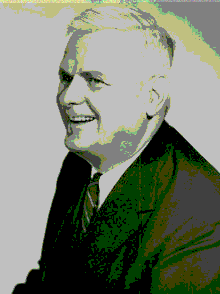
\includegraphics[width=\linewidth]{img/Haskell_6}
		\caption{Шифрование текста в 6 битов байта}
	\end{minipage}
	\hspace{0.02\textwidth}
	\begin{minipage}{0.3\textwidth}
		\centering
		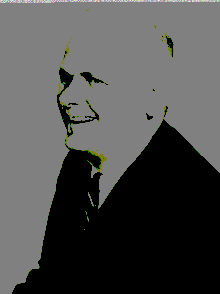
\includegraphics[width=\linewidth]{img/Haskell_7}
		\caption{Шифрование текста в 7 битов байта}
	\end{minipage}
	\hspace{0.02\textwidth}
	\begin{minipage}{0.3\textwidth}
		\centering
		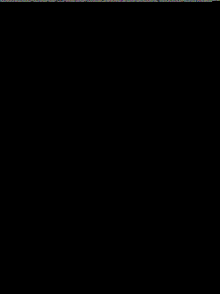
\includegraphics[width=\linewidth]{img/Haskell_8}
		\caption{Шифрование текста в 8 битов байта}
	\end{minipage}
\end{figure}

Как можно заметить, чем большее количество битов в каждом байте используется для записи текста,тем сильнее изменяется изображение.
\newpage

\section* {Заключение}
\addcontentsline{toc}{section}{Заключение}
В ходе выполнения практической работы был создан проект в \texttt{stack}, все чистые функции были записаны \texttt{Lib.hs} и был ограничен доступ к вспомогательным функциям. Использована do-нотация для работы с файлами. Были использованы портрет и биография Алонзо Черча. Была реализована функция шифрующая изображения в текст с помощью шифра с использованием кодового слова, а также реализована функция записывающая текст в последний бит, последние два бита, ..., все биты каждого байта изображения.



\newpage
%\section*{Список литературы}
%\addcontentsline{toc}{section}{Список литературы} % Добавляем раздел в содержание

\begin{thebibliography}{99}
	
	\bibitem{kurtz2019}
	Курт У. \textit{Программируй на Haskell} / пер. с англ. С. Соловьева. — Москва: ДМК Пресс, 2019. — 384 с.
		
	\bibitem{church}
	Church A. Alan Mathison Church. Биография // MacTutor History of Mathematics Archive. URL: \href{https://mathshistory.st-andrews.ac.uk/Biographies/Church/}{https://mathshistory.st-andrews.ac.uk/Biographies/Church/} (дата обращения: 01.12.2024).
	
\end{thebibliography}

\addcontentsline{toc}{section}{Список литературы} % Добавляем раздел в содержание




\end{document}